\documentclass[]{article}

\usepackage{color}
\usepackage[dvipsnames]{xcolor}
\usepackage{tikz}

\usepackage{pgfplots}

\begin{document}

\section{Mise en \oe{uvre}}
\subsection{Impl\'ementation et Analyse de complexit\'e exp\'erimentale}

\subsubsection{Question 4.2}

Les fonctions \texttt{cout1}, \texttt{sol1} et \texttt{cout2} sont programm\'ees en C et contenues dans les fichiers \texttt{cout\_sol\_1.c} et \texttt{cout\_2.c} (en-t\^etes : \texttt{cout\_sol\_1.h}, \texttt{cout\_2.h}). Le jeu d'essai est fourni dans le fichier \texttt{prod.c}. Le \texttt{Makefile} fourni permet de compiler tous les fichiers du projet avec l'utilitaire \texttt{make}, sur toute version de \texttt{gcc} supportant le standard C11.

\subsubsection{Question 4.4}

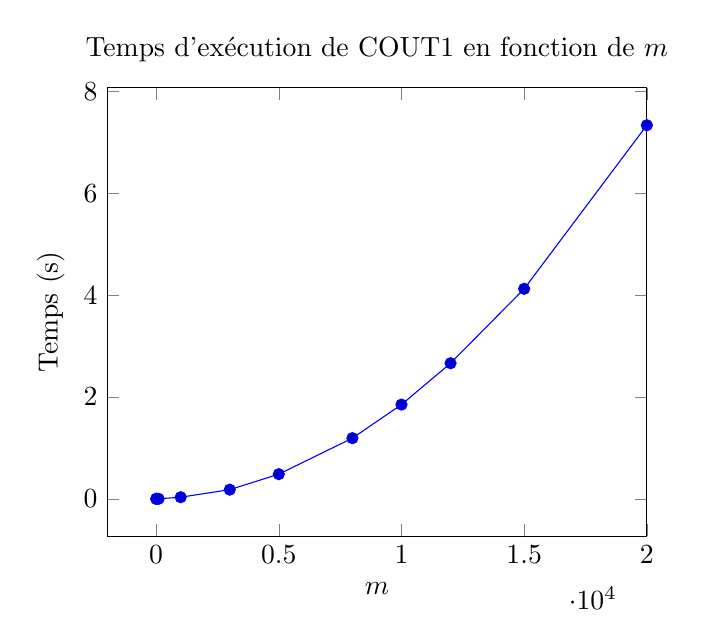
\begin{tikzpicture}
\begin{axis}[xmax=20000,
xlabel={$m$},
ylabel={Temps (s)},
title={Temps d'ex\'ecution de COUT1 en fonction de $m$}]
\addplot coordinates {
(4,0.001) (10,0.0012) (100,0.0018) (1000,0.0328) (3000,0.1812) (5000,0.4856) (8000,1.1926) (10000,1.8514) (12000,2.664) (15000,4.1254) (20000,7.337)};
\end{axis}
\end{tikzpicture}

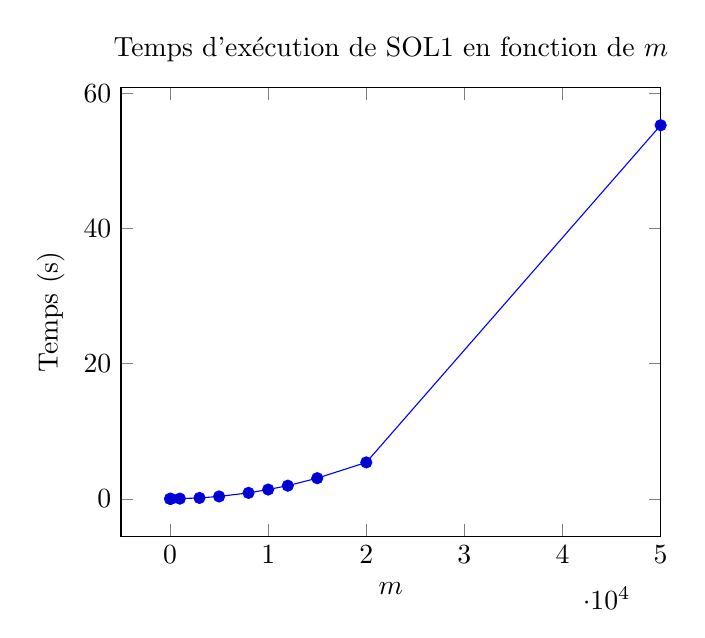
\begin{tikzpicture}
\begin{axis}[xmax=50000,
xlabel={$m$},
ylabel={Temps (s)},
title={Temps d'ex\'ecution de SOL1 en fonction de $m$}]
\addplot coordinates {
(4,0.001) (10,0.0012) (100,0.0012) (1000,0.0294) (3000,0.134) (5000,0.3508) (8000,0.8816) (10000,1.376) (12000,1.9486) (15000,3.0548) (20000,5.3898) (50000,55.2776)};
\end{axis}
\end{tikzpicture}

\subsubsection{Question 4.5}

Pour la fonction \texttt{cout1}, la plus grande valeur de $m$ traitable (en un temps raisonnable d'environ $7,337$ secondes) est $20000$ (\texttt{Inst\_0020000\_64.adn}). Elle est de $50000$ pour la fonction \texttt{sol1} (sans affichage de l'alignement obtenu) pour un temps d'ex\'ecution d'environ $52,4$ secondes.\\Caract\'eristiques m\'emoire de la machine : $8$Go

\subsubsection{Question 4.6}

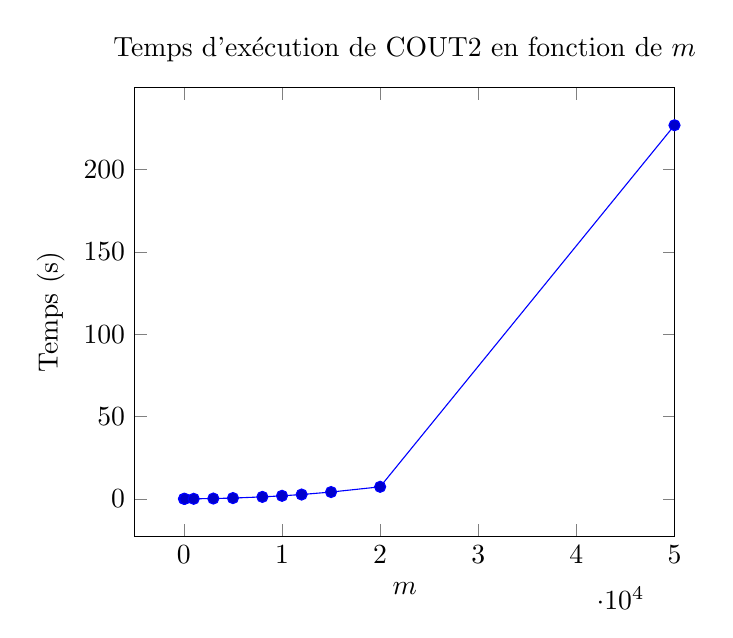
\begin{tikzpicture}
\begin{axis}[xmax=50000,
xlabel={$m$},
ylabel={Temps (s)},
title={Temps d'ex\'ecution de COUT2 en fonction de $m$}]
\addplot coordinates {
(4,0.001) (100,0.0012) (1000,0.0208) (3000,0.1772) (5000,0.465) (8000,1.1818) (10000,1.8282) (12000,2.6134) (15000,4.12) (20000,7.2986) (50000,226.8712)};
\end{axis}
\end{tikzpicture}

Pour la fonction \texttt{cout2}, la plus grande valeur de $m$ traitable est $50000$ (\texttt{Inst\_0050000\_88.adn}); le temps d'ex\'ecution correspondant est d'environ $3,78$ minutes.\\

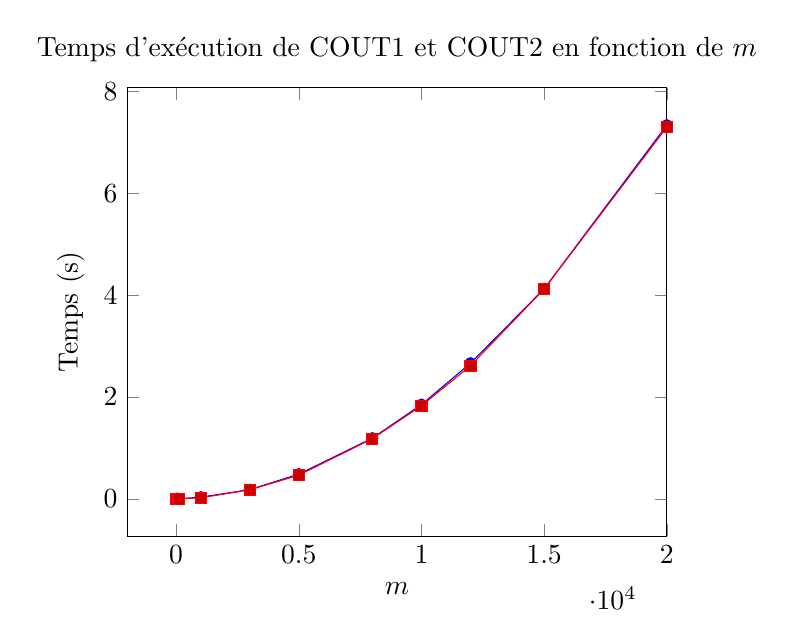
\begin{tikzpicture}
\begin{axis}[xmax=20000,
xlabel={$m$},
ylabel={Temps (s)},
title={Temps d'ex\'ecution de COUT1 et COUT2 en fonction de $m$}]
\addplot coordinates {
(4,0.001) (10,0.0012) (100,0.0018) (1000,0.0328) (3000,0.1812) (5000,0.4856) (8000,1.1926) (10000,1.8514) (12000,2.664) (15000,4.1254) (20000,7.337)};
\addplot coordinates {
(4,0.001) (100,0.0012) (1000,0.0208) (3000,0.1772) (5000,0.465) (8000,1.1818) (10000,1.8282) (12000,2.6134) (15000,4.12) (20000,7.2986)};
\end{axis}
\end{tikzpicture}

\end{document}